%%%%%%%%%%%%%%%%%%%%%%%%%%%%%%%%%%%%%%%%%%%%%%%%%%%%%%%%%%%%%%%%%%%%%%%%%%%%%%%%
%2345678901234567890123456789012345678901234567890123456789012345678901234567890
%        1         2         3         4         5         6         7         8

\documentclass[letterpaper, 10 pt, conference]{ieeeconf}  % Comment this line out
                                                          % if you need a4paper
%\documentclass[a4paper, 10pt, conference]{ieeeconf}      % Use this line for a4
                                                          % paper

\IEEEoverridecommandlockouts                              % This command is only
                                                          % needed if you want to
                                                          % use the \thanks command
\overrideIEEEmargins
% See the \addtolength command later in the file to balance the column lengths
% on the last page of the document



% The following packages can be found on http:\\www.ctan.org
\usepackage{graphicx} % for pdf, bitmapped graphics files
\usepackage{placeins}
\usepackage{listings}
\usepackage{color}

\definecolor{dkgreen}{rgb}{0,0.6,0}
\definecolor{gray}{rgb}{0.5,0.5,0.5}
\definecolor{mauve}{rgb}{0.58,0,0.82}

\lstset{frame=tb,
  language=C,
  aboveskip=3mm,
  belowskip=3mm,
  showstringspaces=false,
  columns=flexible,
  basicstyle={\small\ttfamily},
  numbers=none,
  numberstyle=\tiny\color{gray},
  keywordstyle=\color{blue},
  commentstyle=\color{dkgreen},
  stringstyle=\color{mauve},
  breaklines=true,
  breakatwhitespace=true,
  tabsize=3
}

%\usepackage{epsfig} % for postscript graphics files
%\usepackage{mathptmx} % assumes new font selection scheme installed
%\usepackage{times} % assumes new font selection scheme installed
%\usepackage{amsmath} % assumes amsmath package installed
%\usepackage{amssymb}  % assumes amsmath package installed

\title{\LARGE \bf
Teachable Robotic Grasping Device
}

%\author{ \parbox{3 in}{\centering Huibert Kwakernaak*
%         \thanks{*Use the $\backslash$thanks command to put information here}\\
%         Faculty of Electrical Engineering, Mathematics and Computer Science\\
%         University of Twente\\
%         7500 AE Enschede, The Netherlands\\
%         {\tt\small h.kwakernaak@autsubmit.com}}
%         \hspace*{ 0.5 in}
%         \parbox{3 in}{ \centering Pradeep Misra**
%         \thanks{**The footnote marks may be inserted manually}\\
%        Department of Electrical Engineering \\
%         Wright State University\\
%         Dayton, OH 45435, USA\\
%         {\tt\small pmisra@cs.wright.edu}}
%}

\author{Tariq Zahroof% <-this % stops a space
\thanks{Stanford University:
        {\tt tzahroof@stanford.edu}}%
}


\begin{document}



\maketitle
\thispagestyle{empty}
\pagestyle{empty}


%%%%%%%%%%%%%%%%%%%%%%%%%%%%%%%%%%%%%%%%%%%%%%%%%%%%%%%%%%%%%%%%%%%%%%%%%%%%%%%%
\begin{abstract}

We created a device capable of learning an applied, grasping force and then replicating said force onto a small object. This project serves as a stepping stone to eventually create mobile grasping devices.

\end{abstract}


%%%%%%%%%%%%%%%%%%%%%%%%%%%%%%%%%%%%%%%%%%%%%%%%%%%%%%%%%%%%%%%%%%%%%%%%%%%%%%%%
\section{Introduction}

The objective of the project was to teach a device how to grasp an object by physically demonstrating the proper forces required. The idea was inspired from the way that parents teach their own children. Imagine trying to teach a four-year old how to open the notoriously well-sealed pasta sauce bottle: the mentor would place their hands on top of the child's hands and then apply the appropriate forces and technique to (hopefully) open the bottle. Children learn from application, and we hoped to apply the same idea to this project: teach a robot to grasp by grasping the object with the robot, in hand, first.

This project is a proof-of-concept to demonstrate the capabilities of such a technology. As such, the grasping device is simplistic and is composed of a motor, two 3D-printed grippers, a force sensor, and an Arduino for control. Ultimately, the created device (tethered to a power supply) could apply up to 80 grams of force in order to hold onto an object.



%%%%%%%%%%%%%%%%%%%%%%%%%%%%%%%%%%%%%%%%%%%%%%%%%%%%%%%%%%%%%%%%%%%%%%%%%%%%%%%%
\section{Brainstorming}

Multiple ideas were fielded before I selected the motor-controlled concept. In fact, the project was inspired by the surgeon's hemostat, which clamps the incision together to control bleeding. It uses a ratcheting design by a series of interlocking teeth to lock into place, thus holding the blood vessels together. The design would have likely been motorized to reapply the same forces to differing surfaces. When a sensor between the two pinching arms senses the appropriate force, it would stop applying any additional force. As such, the device would be able to grab objects of different scale.. While conceptually more simple, the resulting design would have required proper material selection and challenging engineering to ensure proper functioning of the teeth (a task which is fairly difficult, but doable, with 3D printing).

Multiple versions of the gripper were brainstormed, using pulleys and gears near the base to move the motor weight away from the force application. However, since the project was simply a proof-of-concept, it was ultimately decided that a simpler prototype using a fixed arm and a motor attached to a movable arm would suffice. The motor would be controlled by a PID system to smoothly apply the needed forces without damaging the object. Ideally, the grasping device would be able to hold any type of surface with as little force as needed, so as not to damage the object. The brainstormed ideas are listed in the appendix.

I used a force sensor resistor to measure the forces applied by the grippers. The sensors were cheap (about \$6 per resistor), had a linear relationship between voltage measured to force applied, and had accuracy to 10N. Furthermore, its thinness easily allowed it to be attached to the flat sides of the arms.


%%%%%%%%%%%%%%%%%%%%%%%%%%%%%%%%%%%%%%%%%%%%%%%%%%%%%%%%%%%%%%%%%%%%%%%%%%%%%%%%
\section{Design}

The motor, found in the lab bins, was mounted to a plate via screw-holes. Then, a movable arm was attached to the motor shaft. The arm was secured by friction by pinching the back end with a nut and bolt. The other arm was tightly attached to the plate by a screw and a nut, preventing movement of the arm when fully setup but allowing re-calibration when need be. Finally, the plate had a slight cubic indentation towards the edge to constrict the arm and prevent it from opening too far. The force resistor was hot glued onto the arm.

\begin{figure}[!htb]
	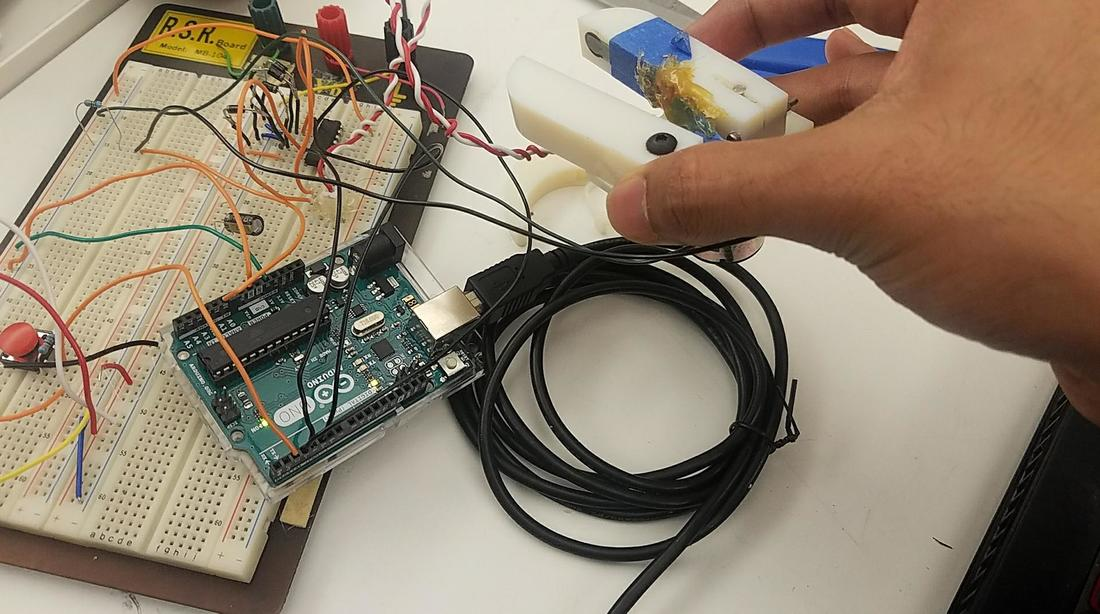
\includegraphics[width=\linewidth]{grasping_device_real_life.jpg}
	\caption{The Final Gripping Device}
	\label{fig:real_life}
\end{figure}
\FloatBarrier

%%%%%%%%%%%%%%%%%%%%%%%%%%%%%%%%%%%%%%%%%%%%%%%%%%%%%%%%%%%%%%%%%%%%%%%%%%%%%%%%

\section{Electronics}

The appendix features the electrical schematic for the device. The force resistor works by a voltage divider and the motor was powered by a L293NE H-bridge (with external snubbing diodes). A button, grounded by a resistor, was used to set the force. The Arduino provided power to the both the resistor and the H-bridge, while a voltage supplier provided 12V at 0.5A to the motor (based on the motor's specifications).



%\addtolength{\textheight}{-3cm}   % This command serves to balance the column lengths
                                  % on the last page of the document manually. It shortens
                                  % the textheight of the last page by a suitable amount.
                                  % This command does not take effect until the next page
                                  % so it should come on the page before the last. Make
                                  % sure that you do not shorten the textheight too much.

%%%%%%%%%%%%%%%%%%%%%%%%%%%%%%%%%%%%%%%%%%%%%%%%%%%%%%%%%%%%%%%%%%%%%%%%%%%%%%%%
%%%%%%%%%%%%%%%%%%%%%%%%%%%%%%%%%%%%%%%%%%%%%%%%%%%%%%%%%%%%%%%%%%%%%%%%%%%%%%%%
\section{Code}

The Arduino code used a state-machine to progress through the functionality of the device. The program would start by passively measuring the applied force. Upon receiving a button press, the arm would open, wait for a little bit, and then start closing. Upon contact with an object surface, the arm would slow down significantly and start applying PID control, where it would perpetually remain until reset (via Arduino). The code is listed in the Appendix.

%%%%%%%%%%%%%%%%%%%%%%%%%%%%%%%%%%%%%%%%%%%%%%%%%%%%%%%%%%%%%%%%%%%%%%%%%%%%%%%%
\section{Observations, Notes, and Thoughts}

The device functioned well, grasping small objects with topographic surfaces. The button, located on the breadboard, was particularly convenient; pressing a button on the actual device proved to be difficult. Unfortunately, the resistor was fairly unreliable, due to the fact that its reading was affected by the geometry of the surface (it recognized pointed surfaces and edges easier than curved surfaces), and that it became damaged if it ever received high forces (which it probably did during the construction phase). The force sensor should be upgraded to something more resilient and more capable of reading a variety of surfaces. Additionally, the motor was not the best for the application; it had a large amount of frictional force (0.7 N) relative to its usual exerted force standard operating conditions (7  N). Its ratio of exerted force to frictional force is fairly low (10) for precise, dexterous applications, and the replacement of said motor with a Maxon counterpart (ratio of around 80) is recommended for future projects. Furthermore, the Arduino should be upgraded to a better microcontroller, as it its timer-interrupt capabilities are limited. I used a PID controller within the loop() function, meaning that all print statements negatively affected the response and the tuning parameters of the PID controller. Finally, the movable arm fixed to the motor shaft still experienced some slippage, despite its pinching fixture, as the bolt and nut slowly lost tension throughout the experiments.

While the above observations are bleak, it is important to remember that the ultimate purpose of this device was to prove the functionality and utility of the idea to create a teachable grasping device. As it turns out, showing something how to hold things is very naturally intuitive and scales relatively well for same masses. Unfortunately, such a strategy neglects to take into account the effects of increased mass of a larger object. The device lacks the capability to scale forces based on object size at the moment.

Continued improvement can also improve on proper grasping technique. The grippers currently glasp with their flat, planar sides in a pinching fashion. This easily allows for objects to slip out. Human fingers tend to curl around objects to provide security along the other axes; adding some similar form of augmentation to the design would guarantee better grasping technique and ensure a better grasp.

Finally, an interesting observation noted during the process is that humans do not intrinsically know the exact force needed to properly pick up an object. Usually, people will increase the force applied as they start lifting the object until there is enough frictional force to hold the object (assuming the person is trying to pinch it upwards and now simply just hold the object). Perhaps, in terms of just picking up and moving objects, an alternative approach would be to explore ways to easily cup and hold objects without having to apply serious frictional forces to maintain the in control of the robot.

%%%%%%%%%%%%%%%%%%%%%%%%%%%%%%%%%%%%%%%%%%%%%%%%%%%%%%%%%%%%%%%%%%%%%%%%%%%%%%%%
\section{Conclusions}

In conclusion, this project was a very satisfying and exciting proof-of-concept work that shows the remarkable potential of a teachable grasping device. Using a simple motor, gripper, force sensor, and PID controller, the device is capable of replicating the grasping forces necessary to pick up and maneuver an object. Used in conjunction with other technologies, such as advanced manipulation and object identification, this device has potential for human-oriented robotics- particularly, human-mounted robotics.

%%%%%%%%%%%%%%%%%%%%%%%%%%%%%%%%%%%%%%%%%%%%%%%%%%%%%%%%%%%%%%%%%%%%%%%%%%%%%%%%
\section{Appendix}

\subsection{Brainstorming}

\begin{figure}[!htb]
	\includegraphics[width=\linewidth]{Brainstorming.pdf}
	\label{fig:brain}
\end{figure}
\FloatBarrier

\begin{figure}[!htb]
	\includegraphics[page=2,width=\linewidth]{Brainstorming.pdf}
	\caption{Brainstorming}
	\label{fig:brain_2}
\end{figure}
\FloatBarrier

\subsection{Design}

\begin{figure}[!htb]
	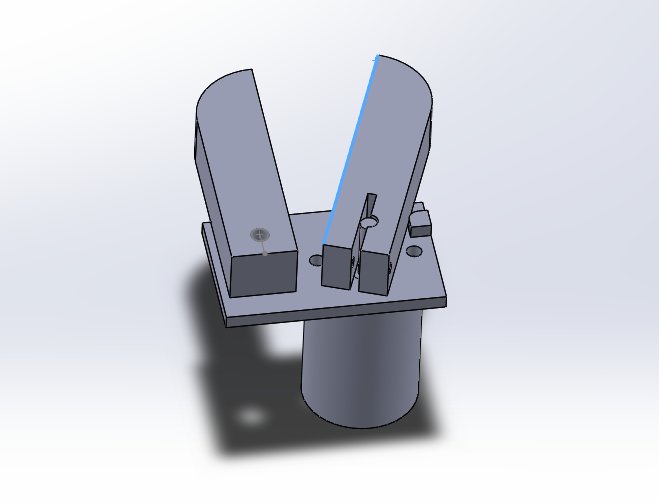
\includegraphics[width=\linewidth]{assembly.png}
	\caption{The Entire Gripping Device}
	\label{fig:assembly}
\end{figure}
\FloatBarrier

\begin{figure}[!htb]
	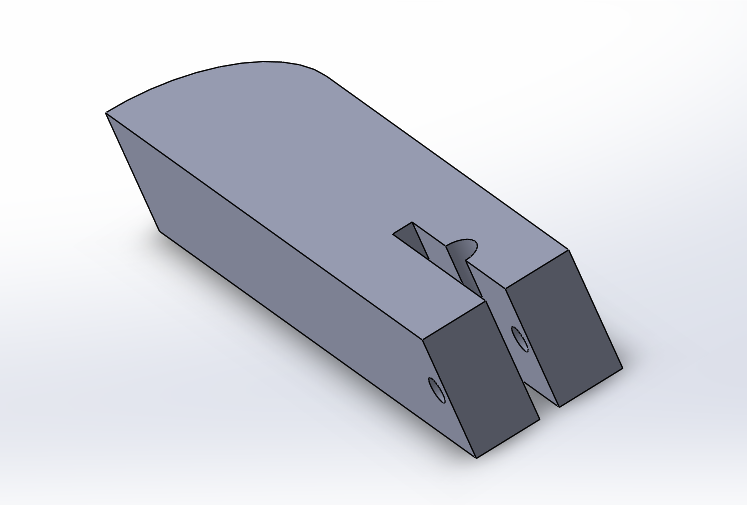
\includegraphics[width=\linewidth]{gripper.png}
	\caption{The Movable Gripper}
	\label{fig:gripper}
\end{figure}
\FloatBarrier

\begin{figure}[!htb]
	\centering
	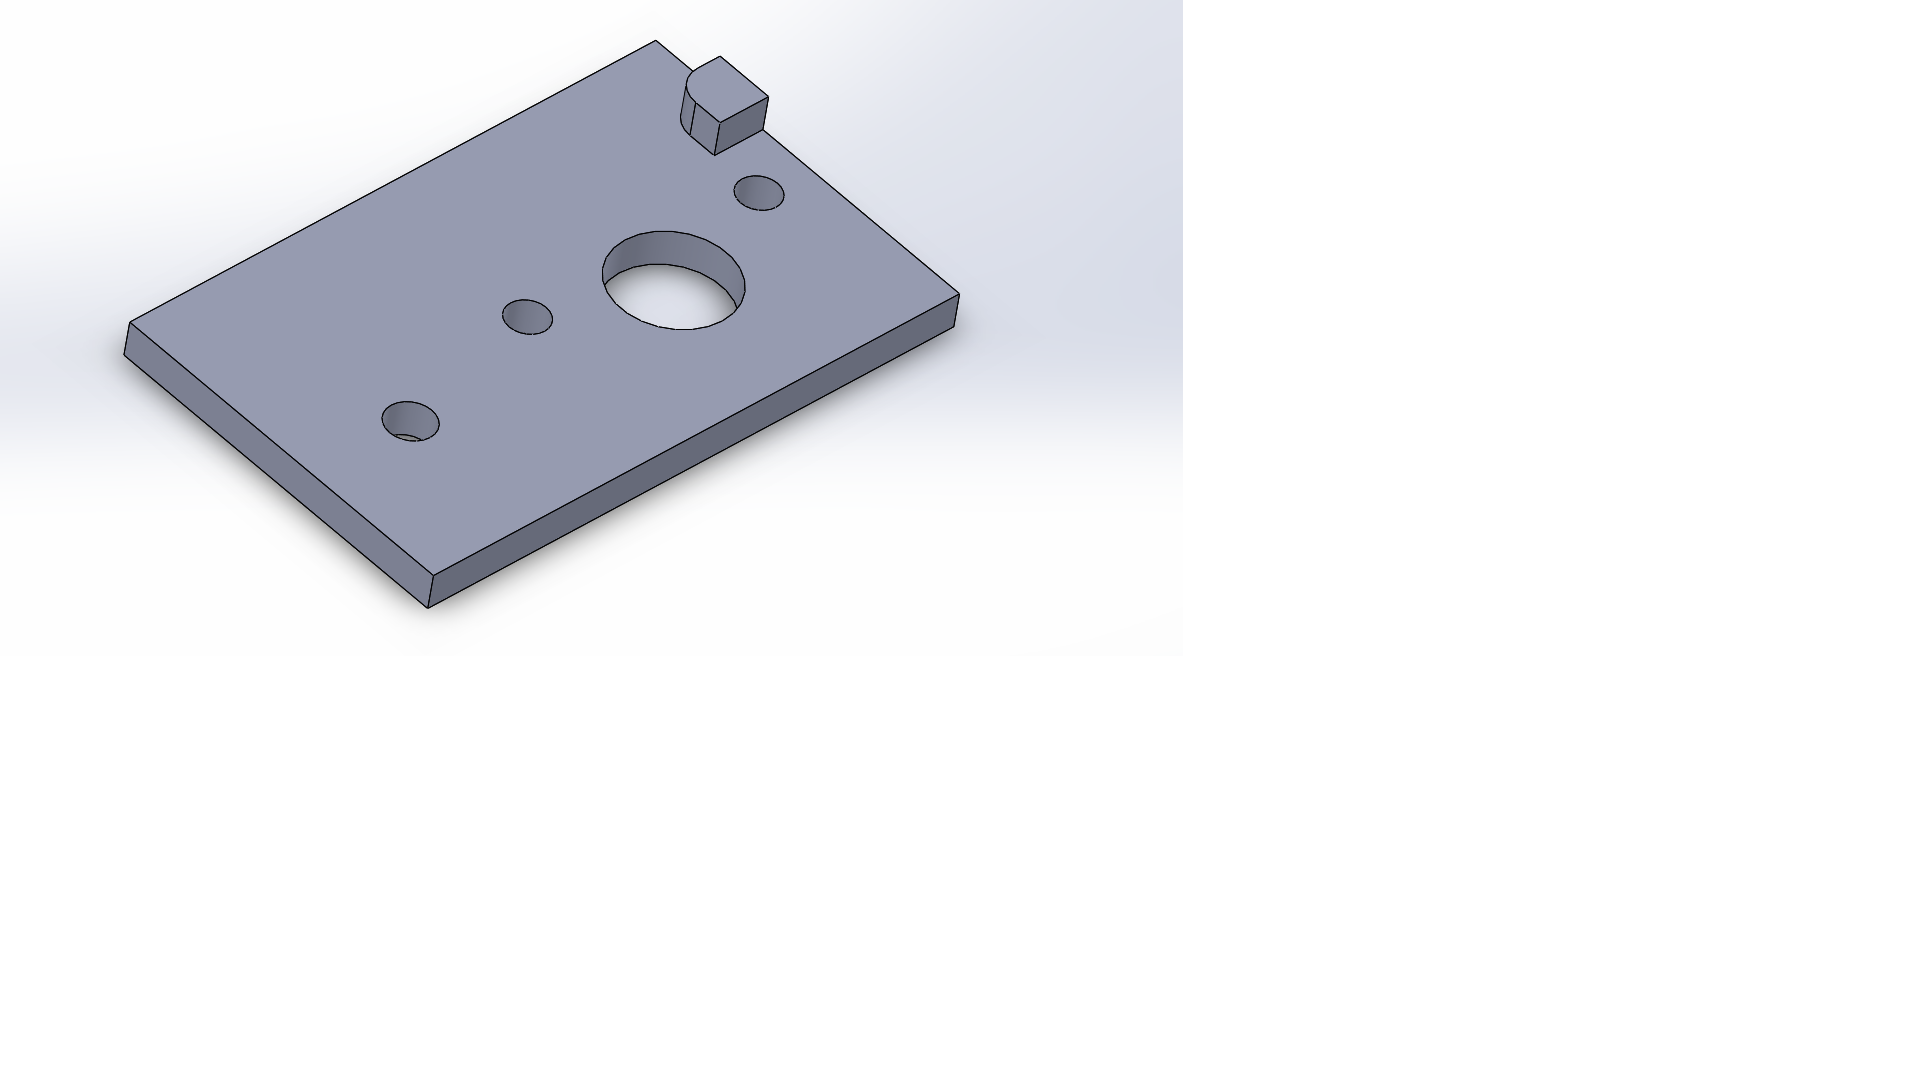
\includegraphics[width=\linewidth]{top_plate.png}
	\caption{The Top Plate}
	\label{fig:top_plate}
\end{figure}
\FloatBarrier

\subsection{Electrical Schematic}

\begin{figure}[!htb]
	\centering
	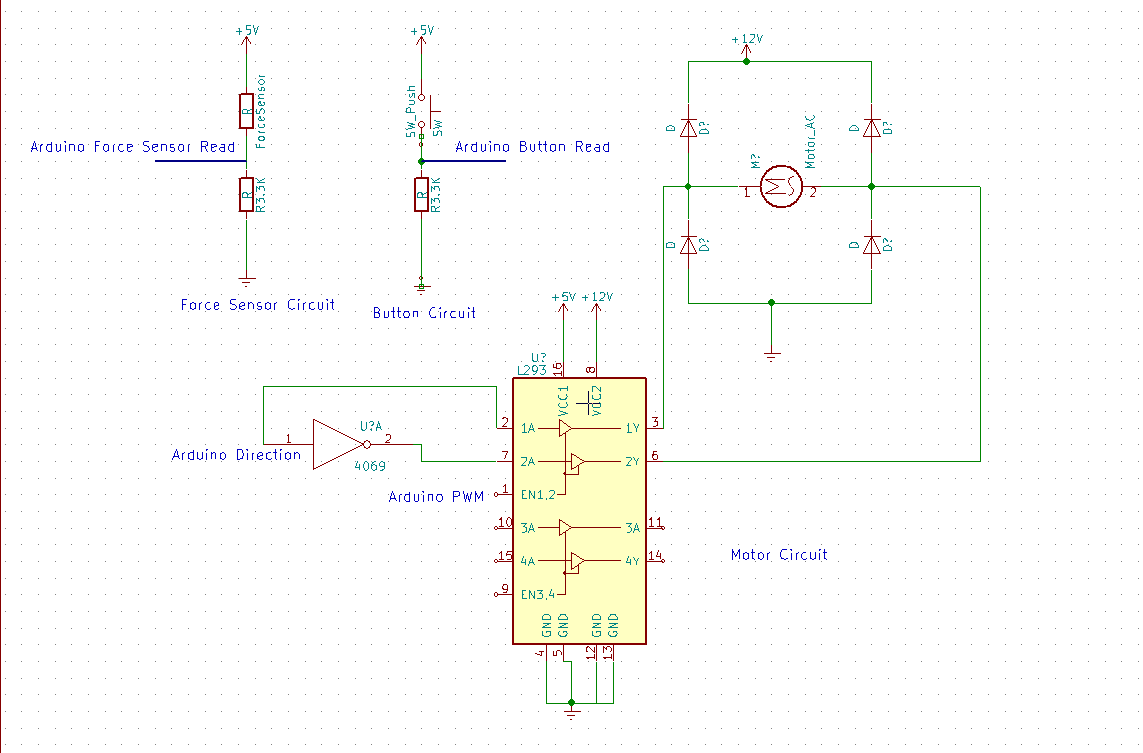
\includegraphics[width=\linewidth]{schematic.png}
	\caption{Electricals Schematic}
	\label{fig:elec}
\end{figure}

\subsection{Code}
\begin{lstlisting}
#include <PID_v1.h>

#define ButtonPin 2
#define ForceSensorPin 0 //ANALOG PIN
#define Direction2Pin 3
#define Direction7Pin 4

#define PWMPin 5
#define RETRACT_TIME 2000 //two seconds

#define forwards HIGH
#define backwards LOW

#define forwardSpeed 150
#define backwardSpeed 200 //between 0 - 255

#define Kp 7
#define Ki 0
#define Kd 1.4//.7

typedef enum {ForceSensing,Retracting, Approaching,Contact} ProjectState;

/*PWM Control Law variables*/
static double PWMControlLaw=0;
static double ForceToRepeat;
static double sumOfErrors  = 0;

static int voltageTicks;
static float VoltageForceSensor = 0;
static float ResistanceForceSensor = 0;
static double Force; // Force that keeps getting updated
static float PeakForce;
static float conductanceForceSensor = 1;
const float VCC = 4.98; //Measured volatege at the Arduino 5V line
const float R_DIV = 3300; //Resistance of a 3.3K resistor

static double prevError = 0;

static ProjectState CurrentState;

void setUpForceResistor() {
  voltageTicks = analogRead(ForceSensorPin);
  PeakForce = 0;
  ForceToRepeat = 0;
}

void setUpMotors(void) {
  pinMode(Direction2Pin, OUTPUT);
  pinMode(Direction7Pin, OUTPUT);

  //ensure that the motors don't spin during start up
  digitalWrite(Direction2Pin, LOW);
  digitalWrite(Direction7Pin, LOW); 
}

void setup() {
  //set up force resistor
  setUpForceResistor();

  //set up button
  pinMode(ButtonPin, INPUT);
  //default assume button low = off

  //set up motors
  setUpMotors();

  //Set CurrentState
  CurrentState = ForceSensing;

  //Start Screen communication
  Serial.begin(9600);
  
}

void VoltageToForce(){
  voltageTicks = analogRead(ForceSensorPin); 
  if(voltageTicks != 0) {
    // use ADC reading to calculate voltage
    VoltageForceSensor = VCC * voltageTicks / 1023.0;
    ResistanceForceSensor = R_DIV *(VCC / VoltageForceSensor - 1);

//    Serial.println("Resistance:: " + String(ResistanceForceSensor) + " ohms");

    conductanceForceSensor = 1.0 / ResistanceForceSensor;

    if(ResistanceForceSensor <= 600){
      Force = (conductanceForceSensor - 0.00075) / 0.00000032639;
    } else {
      Force = conductanceForceSensor / 0.000000642857;
    }
    
    //convert gram force to Newtons
    //Force = Force * .00980665;

   if(CurrentState == ForceSensing) { 
      Serial.println("F: " + String(Force));
   }
//    Serial.println("Set: "+ String(ForceToRepeat)); 
//    Serial.println();
    

  } else {
    //no pressure detected, so do nothing
//    Serial.println("No pressure detected!! ");
//    Serial.println();
    Force = 0;
  }
}

void ApproachAction() {
  digitalWrite(Direction2Pin, HIGH);
  digitalWrite(Direction7Pin, LOW);
  analogWrite(PWMPin, forwardSpeed);
  Serial.println("completed Approach action");
}

void RetractAction() {
  digitalWrite(Direction2Pin, LOW);
  digitalWrite(Direction7Pin, HIGH);
  analogWrite(PWMPin, backwardSpeed);
  Serial.println("Completed Retract action");
}

bool CheckForButton(void) {
  if(digitalRead(ButtonPin)== 0) {
    return false;
  } else {
    return true;
  }
}

void SetDirection(bool dir) {
  //dir == 1 = forwards,
  //dir == 0 = backwards
  if(dir) {
    digitalWrite(Direction2Pin, HIGH);
    digitalWrite(Direction7Pin, LOW);
  } else {
    digitalWrite(Direction2Pin, LOW);
    digitalWrite(Direction7Pin, HIGH);
  }
}


bool CheckForContact() {
  voltageTicks = analogRead(ForceSensorPin);
  Serial.println(voltageTicks);
  if(voltageTicks >= 3) { //ensure that noise is eliminated
    Serial.println("Contact has occurred!");
    VoltageToForce();
    return true;
  }
  return false;
}

void StartTariqControlLaw(void) {
  analogWrite(PWMPin, PWMControlLaw);
  Serial.println("Finished Start Tariq Control Law");
}

void loop() {
  // put your main code here, to run repeatedly:
  switch(CurrentState){
    case ForceSensing:
      if(CheckForButton()) {
       CurrentState = Retracting;
       ForceToRepeat = Force + 5; //give it a slightly higher setpoint
      }
      break;
    case Retracting:
      Serial.println("Doing RETRACTING ACTION");
      RetractAction();
      delay(RETRACT_TIME);
      Serial.println("Finished timeout. Doing Approach Action");
      CurrentState = Approaching;
      ApproachAction();
      break;
    case Approaching:
      if(CheckForContact()) {
        CurrentState = Contact;
//        StartControlLaw();
        StartTariqControlLaw();
      }
      break;
    case Contact:
      //update the PWM based on Control Law
      double error = ForceToRepeat - Force;
      sumOfErrors += error;
      PWMControlLaw = (error * Kp) + (sumOfErrors *Ki) + (error-prevError) * Kd;
//      Serial.print("error: : ");
//      Serial.println(error);
//      Serial.print("PWMControlLaw :: ");
//      Serial.println(PWMControlLaw);
      if(PWMControlLaw >255){
        PWMControlLaw = 255;
      }
      if(PWMControlLaw <-255) {
        PWMControlLaw = -255;
      }
//      Serial.print("PWMControlLaw after clamping:: ");
//      Serial.println(PWMControlLaw);
      if(PWMControlLaw >= 0) {
        SetDirection(true);
        analogWrite(PWMPin, PWMControlLaw);
      } else{
        SetDirection(false);
        analogWrite(PWMPin, -1*PWMControlLaw);
      }
//      Serial.print("Doing Control Law. PWMControlLaw: ");
//      Serial.println(PWMControlLaw);
//      Serial.print("ForceToRepeat SetPoint :: " );
//      Serial.println(ForceToRepeat);
//      Serial.print("error :: ");
      Serial.println(error);
//      Serial.print("Force :: ");
//      Serial.println(Force);


        prevError = error;

      break;
  }
  if(CurrentState != Retracting && CurrentState != Approaching) {
      VoltageToForce(); //keep updating the force sensor
  }

}
\end{lstlisting}


%\bibliographystyle{unsrt} 
%\bibliography{Biblio}  





\end{document}
